%%%%%%%%%%%%%%%%%%%
%  placeholders
%%%%%%%%%%%%%%%%%%%

% chair name not allowed at Department of Informatics
% remove \phantom{} if you want the chair name on the cover
\newcommand{\chair}{\phantom{Lehrstuhl f\"ur Musterverfahren}}
\newcommand{\faculty}{School of Computation, Information and Technology - Informatics}
\newcommand{\uni}{Technical University of Munich}
\newcommand{\studycourse}{Informatics: Games Engineering}

\newcommand{\authorname}{Lukas Jonsson}
\newcommand{\city}{Munich}

\newcommand{\worktype}{Bachelor's Thesis in \studycourse}
\newcommand{\titleFirstLanguage}{Blockchain and Games: Evaluating Practicality and Impact}
% German & English needed at Department of Informatics
\newcommand{\titleForeignLanguage}{Blockchain und Spiele: Bewertung der Anwendbarkeit und Wirkung}

\newcommand{\supervisor}{Prof. Gudrun Klinker, Ph.D.}
\newcommand{\advisor}{Sandro Weber, Ph.D.}

% set date manually or use \today
\newcommand{\submissionDate}{March 15, 2024}



%%%%%%%%%%%%%%%%%%%
%    settings
%%%%%%%%%%%%%%%%%%%

% quick settings
\def\printstyle{twoside} % set to {twoside} for printing, else {oneside}
%\def\monochromeCover{} % uncomment if you prefer a black TUM logo on the cover
%\def\monochromeCoverInside{} % uncomment if you prefer a black TUM logo on the inside cover page

% complete settings & packages: see settings.text

%%%%%%%%%%%%%%%%%%%
% essentials
%%%%%%%%%%%%%%%%%%%

% use the scrbook KOMA document class
\documentclass[	pdftex, 		%
		a4paper, 		% DIN A4 format
		titlepage,		% separate title page
		%draft,			% draft version, no figures in PDF!
		final,			% final version
		\printstyle ,		% see \def in main document (oneside or twoside)
		11pt,			% font size
		DIV=calc,
]{scrbook}
						
\setkomafont{disposition}{\normalfont\bfseries}
\usepackage{scrhack}

% Used to clear empty pages
\let\cleardoublepage\clearpage

% page geometry - define custom if needed...
\def\coverborderleft{20mm} % needed for title page - update: Druck mit Pappumschlag braucht's eher nicht
\usepackage[left=30mm , right=30mm, top=30mm, bottom=30mm]{geometry}

% typesetting
\usepackage{palatino} 				% Palatino font with sans-serif \sffamily Helvetica
\usepackage[utf8]{inputenc} 			% Umlaute
\usepackage[T1]{fontenc}			% extended character set
\parindent0pt           			% no indentation of the first line
\parskip1ex             			% gap between paragraphs
\usepackage{setspace}				% package for line spacing settings
\singlespacing					% 1,0
%\onehalfspacing				% 1,5
%\doublespacing					% 2,0

% language for automated stuff, like "List of Figures" or "Abbildungsverzeichnis"
\usepackage[english]{babel}
%\usepackage[german=quotes]{csquotes} % Deutsche Anführungszeichen

% BibTex
\usepackage[numbers]{natbib}
\bibliographystyle{unsrt}



%%%%%%%%%%%%%%%%%%%
% figures & co
%%%%%%%%%%%%%%%%%%%

% graphics and figures
\usepackage{graphicx, tikz, pgfplots}
\graphicspath{{images/}} % additional path(s) for loading images
\usepackage{rotating} % needed for \begin{sidewaysfigure} ... 

% insert PDF files
\usepackage{framed}
\usepackage{pdfpages}
% settings for PDF Pages to accept additonal versioned PDF files
\pdfminorversion=6
\pdfcompresslevel=9
\pdfobjcompresslevel=9

% define custom colors
\usepackage{xcolor}
\definecolor{gray1}{gray}{0.92}
\definecolor{darkgreen}{rgb}{0,0.5,0}
\definecolor{urlLinkColor}{rgb}{0,0,0.5}
\definecolor{LinkColor}{rgb}{0,0,0}
\definecolor{ListingBackground}{rgb}{0.85,0.85,0.85}

\usepackage{color}
\definecolor{LinkColor}{rgb}{0.1,0.1,0.1}
\definecolor{gray}{rgb}{0.4,0.4,0.4}
\definecolor{darkblue}{rgb}{0.0,0.0,0.6}
\definecolor{cyan}{rgb}{0.0,0.6,0.6}
\definecolor{DarkestGray}{rgb}{0.1,0.1,0.1}
\definecolor{DarkGray}{gray}{0.4}
\definecolor{LightGray}{gray}{0.8}
\definecolor{codegreen}{rgb}{0,0.6,0}
\definecolor{codegray}{rgb}{0.5,0.5,0.5}
\definecolor{codeorange}{rgb}{1,0.5,0}
\definecolor{backcolor}{rgb}{0.95,0.95,0.95}
\definecolor{red}{rgb}{1,0,0} 
\definecolor{blue}{rgb}{0,0,0.6}
\definecolor{green}{rgb}{0,0.8,0}
\definecolor{white}{rgb}{1,1,1}
\definecolor{black}{rgb}{0,0,0}
\definecolor{verylightgray}{rgb}{.97,.97,.97}



%%%%%%%%%%%%%%%%%%%
% layout tools
%%%%%%%%%%%%%%%%%%%

% for \textblock on title page
\usepackage[absolute]{textpos}
%\setlength{\TPHorizModule}{1mm}
%\setlength{\TPVertModule}{\TPHorizModule}

% TUM Corporate Design definitions taken from official templates (tum.de/cd)
\newcommand{\UniversitaetLogoBreite}{19mm}
\newcommand{\UniversitaetLogoHoehe}{1cm}
\definecolor{UniversitaetFarbe}{RGB}{0,101,189}

% blindtext generator
\usepackage{lipsum}

% advanced conditionals
\usepackage{pdftexcmds}


%%%%%%%%%%%%%%%%%%%
% math
%%%%%%%%%%%%%%%%%%%

\usepackage{amssymb}
\usepackage{amsmath}
% custom argmin, argmax
\newcommand{\argmax}[1]{\underset{#1}{\operatorname{arg}\,\operatorname{max}}\;}
\newcommand{\argmin}[1]{\underset{#1}{\operatorname{arg}\,\operatorname{min}}\;}



%%%%%%%%%%%%%%%%%%%
% code listings
%%%%%%%%%%%%%%%%%%%
\usepackage{colortbl}
\usepackage{url}
\usepackage{listings}
%
\usepackage{etoolbox}

\definecolor{base0}{RGB}{131,148,150}
\definecolor{base01}{RGB}{88,110,117}
\definecolor{base2}{RGB}{238,232,213}
\definecolor{sgreen}{RGB}{133,153,0}
\definecolor{sblue}{RGB}{38,138,210}
\definecolor{scyan}{RGB}{42,161,151}
\definecolor{smagenta}{RGB}{211,54,130}


\newcommand\digitstyle{\color{smagenta}}
\newcommand\symbolstyle{\color{base01}}
\makeatletter
\newcommand{\ProcessDigit}[1]
{%
  \ifnum\lst@mode=\lst@Pmode\relax%
   {\digitstyle #1}%
  \else
    #1%
  \fi
}
\makeatother


\lstdefinestyle{solarizedcsharp} {
  language=[Sharp]C,
  frame=lr,
  linewidth=160mm,
  breaklines=true,
  tabsize=2,
  numbers=left,
  numbersep=5pt,
  firstnumber=auto,
  numberstyle=\tiny\ttfamily\color{base0},
  rulecolor=\color{base2},
  basicstyle=\footnotesize\ttfamily,
  commentstyle=\color{base01},
  morecomment=[s][\color{base01}]{/*+}{*/},
  morecomment=[s][\color{base01}]{/*-}{*/},
  morekeywords={  abstract, event, new, struct,
                as, explicit, null, switch,
                base, extern, object, this,
                bool, false, operator, throw,
                break, finally, out, true,
                byte, fixed, override, try,
                case, float, params, typeof,
                catch, for, private, uint,
                char, foreach, protected, ulong,
                checked, goto, public, unchecked,
                class, if, readonly, unsafe,
                const, implicit, ref, ushort,
                continue, in, return, using,
                decimal, int, sbyte, virtual,
                default, interface, sealed, volatile,
                delegate, internal, short, void,
                do, is, sizeof, while,
                double, lock, stackalloc,
                else, long, static,
                enum, namespace, string, var},
  keywordstyle=\bfseries\color{sgreen},
  showstringspaces=false,
  stringstyle=\color{scyan},
  identifierstyle=\color{sblue},
  extendedchars=true,
  literate=
    {0}{{{\ProcessDigit{0}}}}1
    {1}{{{\ProcessDigit{1}}}}1
    {2}{{{\ProcessDigit{2}}}}1
    {3}{{{\ProcessDigit{3}}}}1
    {4}{{{\ProcessDigit{4}}}}1
    {5}{{{\ProcessDigit{5}}}}1
    {6}{{{\ProcessDigit{6}}}}1
    {7}{{{\ProcessDigit{7}}}}1
    {8}{{{\ProcessDigit{8}}}}1
    {9}{{{\ProcessDigit{9}}}}1
    {\}}{{\symbolstyle{\}}}}1
    {\{}{{\symbolstyle{\{}}}1
    {(}{{\symbolstyle{(}}}1
    {)}{{\symbolstyle{)}}}1
    {=}{{\symbolstyle{$=$}}}1
    {;}{{\symbolstyle{$;$}}}1
    {>}{{\symbolstyle{$>$}}}1
    {<}{{\symbolstyle{$<$}}}1
    {\%}{{\symbolstyle{$\%$}}}1,
}

\lstset{escapechar=@,style=solarizedcsharp}
%% Copyright 2017 Sergei Tikhomirov, MIT License
% https://github.com/s-tikhomirov/solidity-latex-highlighting/

\definecolor{verylightgray}{rgb}{.97,.97,.97}

\lstdefinelanguage{Solidity}{
	keywords=[1]{anonymous, assembly, assert, balance, break, call, callcode, case, catch, class, constant, continue, constructor, contract, debugger, default, delegatecall, delete, do, else, emit, event, experimental, export, external, false, finally, for, function, gas, if, implements, import, in, indexed, instanceof, interface, internal, is, length, library, log0, log1, log2, log3, log4, memory, modifier, new, payable, pragma, private, protected, public, pure, push, require, return, returns, revert, selfdestruct, send, solidity, storage, struct, suicide, super, switch, then, this, throw, transfer, true, try, typeof, using, value, view, while, with, addmod, ecrecover, keccak256, mulmod, ripemd160, sha256, sha3}, % generic keywords including crypto operations
	keywordstyle=[1]\color{blue}\bfseries,
	keywords=[2]{address, bool, byte, bytes, bytes1, bytes2, bytes3, bytes4, bytes5, bytes6, bytes7, bytes8, bytes9, bytes10, bytes11, bytes12, bytes13, bytes14, bytes15, bytes16, bytes17, bytes18, bytes19, bytes20, bytes21, bytes22, bytes23, bytes24, bytes25, bytes26, bytes27, bytes28, bytes29, bytes30, bytes31, bytes32, enum, int, int8, int16, int24, int32, int40, int48, int56, int64, int72, int80, int88, int96, int104, int112, int120, int128, int136, int144, int152, int160, int168, int176, int184, int192, int200, int208, int216, int224, int232, int240, int248, int256, mapping, string, uint, uint8, uint16, uint24, uint32, uint40, uint48, uint56, uint64, uint72, uint80, uint88, uint96, uint104, uint112, uint120, uint128, uint136, uint144, uint152, uint160, uint168, uint176, uint184, uint192, uint200, uint208, uint216, uint224, uint232, uint240, uint248, uint256, var, void, ether, finney, szabo, wei, days, hours, minutes, seconds, weeks, years},	% types; money and time units
	keywordstyle=[2]\color{teal}\bfseries,
	keywords=[3]{block, blockhash, coinbase, difficulty, gaslimit, number, timestamp, msg, data, gas, sender, sig, value, now, tx, gasprice, origin},	% environment variables
	keywordstyle=[3]\color{violet}\bfseries,
	identifierstyle=\color{black},
	sensitive=true,
	comment=[l]{//},
	morecomment=[s]{/*}{*/},
	commentstyle=\color{gray}\ttfamily,
	stringstyle=\color{red}\ttfamily,
	morestring=[b]',
	morestring=[b]"
}

\lstset{
	language=Solidity,
	backgroundcolor=\color{verylightgray},
	extendedchars=true,
	basicstyle=\footnotesize\ttfamily,
	showstringspaces=false,
	showspaces=false,
	numbers=left,
	numberstyle=\footnotesize,
	numbersep=9pt,
	tabsize=2,
	breaklines=true,
	showtabs=false,
	captionpos=b
}

\lstdefinelanguage{Solidity}{
	keywords=[1]{anonymous, assembly, assert, balance, break, call, callcode, case, catch, class, constant, continue, constructor, contract, debugger, default, delegatecall, delete, do, else, emit, event, experimental, export, external, false, finally, for, function, gas, if, implements, import, in, indexed, instanceof, interface, internal, is, length, library, log0, log1, log2, log3, log4, memory, modifier, new, payable, pragma, private, protected, public, pure, push, require, return, returns, revert, selfdestruct, send, solidity, storage, struct, suicide, super, switch, then, this, throw, transfer, true, try, typeof, using, value, view, while, with, addmod, ecrecover, keccak256, mulmod, ripemd160, sha256, sha3}, % generic keywords including crypto operations
	keywordstyle=[1]\color{blue}\bfseries,
	keywords=[2]{address, bool, byte, bytes, bytes1, bytes2, bytes3, bytes4, bytes5, bytes6, bytes7, bytes8, bytes9, bytes10, bytes11, bytes12, bytes13, bytes14, bytes15, bytes16, bytes17, bytes18, bytes19, bytes20, bytes21, bytes22, bytes23, bytes24, bytes25, bytes26, bytes27, bytes28, bytes29, bytes30, bytes31, bytes32, enum, int, int8, int16, int24, int32, int40, int48, int56, int64, int72, int80, int88, int96, int104, int112, int120, int128, int136, int144, int152, int160, int168, int176, int184, int192, int200, int208, int216, int224, int232, int240, int248, int256, mapping, string, uint, uint8, uint16, uint24, uint32, uint40, uint48, uint56, uint64, uint72, uint80, uint88, uint96, uint104, uint112, uint120, uint128, uint136, uint144, uint152, uint160, uint168, uint176, uint184, uint192, uint200, uint208, uint216, uint224, uint232, uint240, uint248, uint256, var, void, ether, finney, szabo, wei, days, hours, minutes, seconds, weeks, years},	% types; money and time units
	keywordstyle=[2]\color{teal}\bfseries,
	keywords=[3]{block, blockhash, coinbase, difficulty, gaslimit, number, timestamp, msg, data, gas, sender, sig, value, now, tx, gasprice, origin},	% environment variables
	keywordstyle=[3]\color{violet}\bfseries,
	identifierstyle=\color{black},
	sensitive=true,
	comment=[l]{//},
	morecomment=[s]{/*}{*/},
	commentstyle=\color{gray}\ttfamily,
	stringstyle=\color{red}\ttfamily,
	morestring=[b]',
	morestring=[b]"
}
\lstloadlanguages{C, C++, csh, Solidity} % add languages if needed 
\lstset{
	language=csh,
	basicstyle=\footnotesize\ttfamily,
	numbers=left,
	numberstyle=\tiny,
	numbersep=5pt,
	tabsize=2,
	extendedchars=true,
	breaklines=true,
	frame=tb,
	stringstyle=\color{codeorange}\ttfamily,
	showspaces=false,
	showtabs=false,
	xleftmargin=17pt,
	framexleftmargin=17pt,
	framexrightmargin=5pt,
	framexbottommargin=4pt,
	commentstyle=\color{codegreen},
	morecomment=[l]{//}, %use comment-line-style!
	morecomment=[s]{/*}{*/}, %for multiline comments
	showstringspaces=false,
	morekeywords={ abstract, event, new, struct,
		as, explicit, null, switch,
		base, extern, object, this,
		bool, false, operator, throw,
		break, finally, out, true,
		byte, fixed, override, try,
		case, float, params, typeof,
		catch, for, private, uint,
		char, foreach, protected, ulong,
		checked, goto, public, unchecked,
		class, if, readonly, unsafe,
		const, implicit, ref, ushort,
		continue, in, return, using,
		decimal, int, sbyte, virtual,
		default, interface, sealed, volatile,
		delegate, internal, short, void,
		do, is, sizeof, while,
		double, lock, stackalloc,
		else, long, static,
		enum, namespace, string, void},
	keywordstyle=\color{blue},
	identifierstyle=\color{black},
	backgroundcolor=\color{white},
}
\lstset{
	language=Solidity,
	backgroundcolor=\color{verylightgray},
	extendedchars=true,
	basicstyle=\footnotesize\ttfamily,
	showstringspaces=false,
	showspaces=false,
	numbers=left,
	numberstyle=\footnotesize,
	numbersep=9pt,
	tabsize=2,
	breaklines=true,
	showtabs=false,
	captionpos=b
}
% captions for listings
\usepackage{caption}
\DeclareCaptionFont{white}{\color{white}}
\DeclareCaptionFormat{listing}{\colorbox[cmyk]{0.43, 0.35, 0.35,0.01}{\parbox{\textwidth}{\hspace{15pt}#1#2#3}}}
\captionsetup[lstlisting]{format=listing,labelfont=white,textfont=white, singlelinecheck=false, margin=0pt, font={footnotesize}}



%%%%%%%%%%%%%%%%%%%
% header & footer
%%%%%%%%%%%%%%%%%%%

\usepackage{fancyhdr}
\pagestyle{fancy}
\fancyhead{}
\fancyfoot{} 
\renewcommand{\headrulewidth}{0.4pt} % line for header - 0.0pt = no line
\renewcommand{\footrulewidth}{0.0pt} % line for footer - 0.0pt = no line

\renewcommand{\chaptermark}[1]{\markboth{\thechapter\quad#1}{}}
\renewcommand{\sectionmark}[1]{\markright{\thesection\quad#1}}

\fancyhead[LO]{\textit{\rightmark}}	
\fancyhead[RO]{\textit{\thepage}}

\def\twoside{twoside} % macro needed
\ifx \printstyle \twoside
	% adapt footers and headers if two-sided
	\fancyhead[LE]{\textit{\thepage}}	
	\fancyhead[RE]{\textit{\rightmark}}
\fi



%%%%%%%%%%%%%%%%%%%
% hyperref
%%%%%%%%%%%%%%%%%%%

\usepackage[
	pdftitle={\titleFirstLanguage},
	pdfauthor={\authorname},
	pdfsubject={\titleFirstLanguage},
	pdfcreator={MiKTeX, LaTeX with hyperref and KOMA-Script based on template by Michael Grupp ( github.com/MichaelGrupp/TTT )},
	pdfkeywords={Abschlussarbeit, Thesis, TUM}, 
	pdfpagemode=UseOutlines,%                                  
	pdfdisplaydoctitle=true,%                                  
	pdflang=de%                                              
]{hyperref}

\hypersetup{%
	colorlinks=true,%        colored links without border
	linkcolor=LinkColor,%    
	citecolor=LinkColor,%    
	filecolor=LinkColor,%    
	menucolor=LinkColor,%    
	urlcolor=LinkColor,%     
	bookmarksnumbered=true%  
}
 







%%%%%%%%%%%%%%%%%%%
%  main document
%%%%%%%%%%%%%%%%%%%

\begin{document}

\frontmatter
% first part of document before actual content

\begin{titlepage}

% Dreizeiler:
\begin{textblock*}{\textwidth}(\coverborderleft, 2cm)%        	
    	\setlength{\baselineskip}{11pt}%
    	\ifx \monochromeCover \undefined
        	\textcolor{UniversitaetFarbe} { %
        	\fontsize{9}{11}\selectfont%
        	\sffamily \chair\\%
        	\sffamily \faculty\\%
        	\sffamily \uni }
    \else
        	\textcolor{black} { %
        	\fontsize{9}{11}\selectfont%
        	\sffamily \chair\\%
        	\sffamily \faculty\\%
        	\sffamily \uni }
    \fi
\end{textblock*}%

% TUM logo
\begin{textblock*}{\UniversitaetLogoBreite}[1,0](\paperwidth - 2cm, 2cm)%
		\ifx \monochromeCover \undefined
        	
\includegraphics{images/TUM_Logos/TUM_blau.pdf}%
        \else
        	
\includegraphics{images/TUM_Logos/TUM_schwarz.pdf}%
        \fi
\end{textblock*}%

% title text
\begin{textblock*}{\paperwidth - \coverborderleft - 2cm}(\coverborderleft , 8cm)% 
\raggedright %no hyphenation here
{\sffamily \Large \worktype}\\
{\sffamily \huge \titleFirstLanguage \par} %~\\[2mm]
\vspace{1cm}
\sffamily \Large \textbf{\authorname}\\
\end{textblock*}

~\\ % do not remove
\end{titlepage}
\begin{titlepage}

% Dreizeiler:
\begin{textblock*}{\textwidth}(\coverborderleft, 2cm)%        	
    	\setlength{\baselineskip}{11pt}%
    	\ifx \monochromeCoverInside \undefined
        	\textcolor{UniversitaetFarbe} { %
        	\fontsize{9}{11}\selectfont%
        	\sffamily \chair\\%
        	\sffamily \faculty\\%
        	\sffamily \uni }
    \else
        	\textcolor{black} { %
        	\fontsize{9}{11}\selectfont%
        	\sffamily \chair\\%
        	\sffamily \faculty\\%
        	\sffamily \uni }
    \fi
\end{textblock*}%

% TUM logo
\begin{textblock*}{\UniversitaetLogoBreite}[1,0](\paperwidth - 2cm, 2cm)%
		\ifx \monochromeCoverInside \undefined
        	
\includegraphics{images/TUM_Logos/TUM_blau.pdf}%
        \else
        	
\includegraphics{images/TUM_Logos/TUM_schwarz.pdf}%
        \fi
\end{textblock*}%

% title in German and English with additional infos
\begin{textblock*}{\paperwidth - \coverborderleft -2cm}(\coverborderleft, 8cm)% 
\raggedright %no hyphenation here
{\sffamily \Large \worktype}\\
{\sffamily \huge \titleFirstLanguage \par}
\vspace{1cm}
{\sffamily \huge \titleForeignLanguage \par}
\end{textblock*}
\begin{textblock*}{\paperwidth - \coverborderleft - 2cm}(\coverborderleft, \paperheight - 5cm)% 
\begin{tabular}{l l}
\sffamily Author: & \sffamily \authorname \\
\sffamily Supervisor: & \sffamily \supervisor \\
\sffamily Advisors: & \sffamily \advisor \\
\sffamily Submission Date: & \sffamily \submissionDate
\end{tabular}
\end{textblock*}

~\\ % do not remove
\end{titlepage} % needed at Department of Informatics

%\newpage\null\thispagestyle{empty}\newpage

\chapter{Eidesstattliche Erkl\"arung}
Ich versichere hiermit, dass ich diese Bachelor's Thesis selbständig verfasst und nur die angegebenen Quellen und Hilfsmittel verwendet habe.
\\[1cm]
I confirm that this bachelor's thesis is my own work and I have documented all sources and material used.
\\[6ex]

\city, \today

\vspace{1.5cm}
\rule[-0.2cm]{5cm}{0.5pt}

\textsc{\authorname} 

\chapter{Abstract}\label{Abstract}
This thesis discusses the practicality and impact of blockchain technologies on game development.
Due to the increasingly popular topic of blockchain, so-called blockchain games have been published in the past.
This raises the question of whether using this technology as a foundation for games is a valid design choice.
In order to understand the arguments, a theoretical basis must first be created. 
To achieve this, we first summarize the historical background of blockchain technology and the development of Bitcoin to understand why it exists and what it is used for. 
After looking closer at the Bitcoin blockchain implementation, we introduce Ethereum and its smart contract capabilities, which are needed to write simple Turing-complete programs that the Ethereum Virtual Machine can execute.
In addition, examples of smart contracts and their usage in the Unity game engine are presented.
The evaluation chapter of this thesis then discusses various arguments for and against blockchain as a tool in software and especially game development.
By reading this work, the reader will gain a deeper understanding of blockchain technology and thus be able to follow and evaluate the arguments in this ongoing discussion.
% \chapter{Acknowledgements}

I would like to thank Michael Grupp for this \LaTeX\ template.

\lipsum[1-2]


\tableofcontents 

%\newpage\null\thispagestyle{empty}\newpage


\mainmatter
% include chapter files here or write your text directly here

\chapter{Motivation}

Computers and the Internet play an essential role in today's world. 
Many things in modern society would only work with digital technology.
Even back in 2004, Hoffman, Novak, and Venkatesh raised the question of whether the Internet has become indispensable, meaning the integration into one's daily life \cite{hoffman2004}.
Nearly two decades later, this question is still relevant.
With a modern computer or mobile phone, one can access publicly available information quickly because every bit of information is copyable on a digital device.
Viewing a website, sending an email, or creating a post on X is only possible by copying data.
However, the fact that every bit is duplicatable creates a new untrivial problem of digital information.
Financial systems rely on the immutability of completed transactions. 
No one would buy a stock if it were just a file that everyone could easily copy.
Spending cash online would not make sense if anyone could duplicate a dollar bill before using it for an online transaction.
The standard way to solve this problem is to establish a trusted third party that would monitor everything and log the rightful owner of the file.
Still, new problems arise when using a system based on trust.

In 2008, Satoshi Nakamoto published a whitepaper to a mailing list of cryptographers on metzdowd.com \cite{nakamotoemail_1}.
The paper is called "Bitcoin: A Peer-to-Peer Electronic Cash System" \cite{nakamoto2008} and proposes a solution to this problem. 
It includes the concept of a digital payment system that uses a so-called blockchain.
This new technology should solve issues of digital cash like double-spending \cite{chowan2021}, privacy, and the need for trusted third parties \cite{Douceur2002}.
The blockchain would not only be used to run the Bitcoin protocol but was also the discovery of digital scarcity.
A bitcoin is not copyable because of the immutability of the transaction record made possible by the blockchain \cite{popovski2014}.
Although, are there other fields of application for this solution?

More than a decade later, many industries are trying to use the blockchain to enhance existing systems, one being the gaming industry \cite{fowler2021}.
As a game developer, the evaluation of the practicality and the impact of blockchain technology in game development raised my interest.
\chapter{History}
It is essential to look at the technological pioneers to understand how blockchains work, what led to their invention, and what they are useful for.
In the 1980s, the \textbf{Cypherpunk movement} emerged.
Inspired by the ideas of David Chaum, they believed in cryptography to weaken the governmental influence in the digital realm.
The use of cryptographic algorithms could enhance people's privacy.
These ideas consequently result in a concept called crypto-anarchism.
While a government enforces laws, crypto-anarchism solely relies on laws written in code and provable by math.
These technologies are essential to guarantee privacy, especially in countries with poor human rights or corruption.
Hence, digital money is also an important research field since money transactions reveal much about the person behind it. \cite{Narayanan2013}

\section{Problems of digital cash}
Over the years, many different concepts were designed to solve the problems of digital cash.
Before looking into these protocols, the problems need to be defined.

\subsection{Double-Spending}
Double-spending describes the situation where money is spent twice simultaneously. 
However, When someone receives money, they must be sure that it belongs to them now and that it was not spent twice at the same time.
This problem is only severe in decentralized networks because a centralized database would know the rightful owners of a money unit at any given moment, thus solving the problem.
Accordingly, when a trusted third party must be excluded, the problem is not trivial anymore.
The network must agree on a network state that contains every user's balances.
Whenever someone performs a money transaction, the state of the network defined by all the data it shares changes.
When the network is distributed across substantial geographical distances, users might issue two transactions simultaneously and spread them to different network parts.
These two parts would then accept different states, which makes reaching a network consensus impossible.
The network must find a solution to problems like this to prevent any double-spending attempts. \cite{chowan2021}

\subsection{Inflation}
When dealing with digital information, every bit is copyable.
Given that the Cypherpunks did not want to use a central database to control the money supply, a solution had to be found to create a form of digital scarcity that no one could control.
If one money unit were a regular file, everyone could copy it before spending it online.
This action would not only inflate the money supply and thus make it worthless but also make double-spending possible.
A suitable protocol must find a way to control the money supply on a decentralized basis.
Therefore, the money creation process must have two properties.
Firstly, it must be unaffected by technological progress.
With faster computers in the future, the algorithm to create money cannot generate more money the faster or more often it is executed.
Secondly, it cannot grant selected network participants exclusive control over it.


\subsection{Byzantine General's Problem}
Inflation and double-spending are solvable problems by agreeing on a network state.
However, in a decentralized network, every user has the same rights.
Consequently, bad actors are also allowed and cannot be banned.
Instead of excluding them, the protocol must be resilient against manipulation or tampering.
The Byzantine Generals Problem is a thought experiment that illustrates this situation.
It describes a scene where the Byzantine army besieges an enemy castle.
The army consists of many small groups of soldiers, each controlled by a general.
In order to win the battle and take the castle, the generals must devise a plan.
Nevertheless, they can only communicate via messengers because they are geographically separated.
Since some generals may be traitors, a consensus mechanism must be found that makes it possible to find a valid strategy as long as most generals are loyal.
In a computer context, the generals are nodes in a distributed network.
The nodes want to reach a consensus on a network state while bad actors are possible.
The resilience against those bad actors influencing a network consensus is called byzantine fault tolerance.
\cite{lamport2019byzantine}

\subsection{Sybil Attack}
The Byzantine general's problem is solvable if there are enough honest nodes in a decentralized network.
Thus, an attacker would try to create many fake identities, make them join the network, and force a different consensus.
This process is called a Sybil attack.
The problem can be solved by designing the protocol to make Sybil attacks very difficult or uneconomical for the attacker.
If the cost of performing an attack would be much higher than the reward, it is much less likely that someone would try to carry out such an attack.
\cite{Douceur2002}

\section{Cryptography}
Besides problems related to digital cash, digital privacy is also an important topic, achievable using modern cryptography.
It describes the information encoding process to a ciphertext so only designated entities can decrypt it back to plaintext.

The beginnings of cryptography go back to early human history.
Even the Greeks used special sticks with tape that would be used to encode a message.
The message could not be recovered if the tape was removed from the stick.
A second example is the Caesar Shift Cipher of the Roman Empire. \cite{Damico2009}

In 1918, Arthur Scherbius invented the Enigma machine to encrypt a message automatically.
The device had three disks. The first would encode a plaintext letter into a cipher letter.
Consequently, the other two disks would repeat the encoding process so that a letter would be encoded three times.
The Allied forces tried to decrypt the machine since the Third Reich used it for military communication during the Second World War.
Alan Turing then cracked the code by inventing machines that could simulate the enigma to decrypt the enemy's communication.
A great help would be that the messages contained military keywords that could be used to search for patterns. \cite{Crato2010}
However, modern-day cryptography is more advanced than the enigma machine. 

First, there is \textbf{symmetrical cryptography}.
It is called symmetrical because a symmetric cryptographic algorithm uses one key to encrypt and decrypt plaintext.
Both the sender and the receiver know the key.

Second, there is \textbf{asymmetric cryptography}.
The critical difference is that it uses key pairs instead of one key.
A key pair consists of a public key that is publicly known and a private key that is only known to its owner.
They are both mathematically related to one another, which makes several calculations possible.
First, a private key can sign data. 
The signature is then verifiable with the public key.
Like a hand signature, cryptographic signatures can be used to verify that the person holding the private key has taken a specific action.
For example, the owner can sign a message and prove that it came from them.
It is further possible to encrypt data with a public key, making it only decryptable by the respective private key.

Third, there are cryptographic functions, called \textbf{hash functions}, that are used for one-way encryption and do not use keys at all.
A primary property of hash functions is that their output, called hash, is unrelated to the input data.
Nevertheless, the same input always produces the same output while avoiding collisions, meaning two identical inputs that result in the same output hash.
One use case for such functions is saving user credentials in a database.
Instead of saving passwords as plaintext, only their hashes are stored.
When a user tries to log into their account, the system recalculates the hash and compares it to the one saved in the database.
\cite{genccouglu2019importance}

\hrule
By using the hash function sha256 with the input Hello world, the following hash value can be generated.
\vspace{4pt}
\begin{equation}
    \textrm{64ec88ca00b268e5ba1a35678a1b5316d212f4f366b2477232534a8aeca37f3c}
\end{equation}

\hrule
\vspace{4pt}

These hashes can be combined into an immutable binary hash tree, called Merkle tree \cite{merkle_tree}.
The result of a Merkle tree creation is the tree's root hash.
The root can be used to verify whether a transaction was added during the tree creation.
Hence, the Merkle tree root serves as a digital fingerprint over the hashes it includes because it cannot be altered after its creation.

\section{Blind Signatures}

In 1982, David Chaum released a paper about a new concept called blind signatures.
He described a payment system that could provide cryptographic proof of payment.
Two main goals were to make payments untraceable and unlinkable.
These targets are achieved by making a bank create cryptographically signed numbers that are usable as monetary units.
A user with a bank account can then withdraw the signed number from the bank and send it to a shop owner as a payment.
At that point, the shop owner would deposit the signed number into their bank account.
As a trusted third party, the bank keeps track of the signed coins without saving personal information and denies the transaction if a coin has already been spent. \cite{chaum1983}

Since every money unit is only a signed number, the bank cannot link it to the user \cite{pointcheval2000}.
Further, some mathematical properties of this concept are defined.
First of all, a trusted third party is needed.
In a digital payment system, a bank would portray this role.
In addition, the three following functions are needed to make the system work.
\begin{itemize}
    \item A signing function \textbf{s'} that is only known to the bank and its publicly known inverse function \textbf{s}.
    \item A commuting function \textbf{c} and its inverse function \textbf{c'} which are both only known to the payer.
    \item A predicate \textbf{r} used to check for redundancy
\end{itemize}
Chaum describes the system as follows.
In order to send money from the payer to a shop, they need a certificate \textbf{x} signed by the bank that contains the amount of money they want to spend.
Since the system is designed to provide anonymity to the payer, they encrypt \textbf{x} using their commuting function \textbf{c}.
\begin{equation}
    c\left(x\right) = enc\left(x\right)~.
\end{equation}
They then send it to the bank, which uses its signing function to sign the amount using \textbf{s'}.
\begin{equation}
    s'\left(enc\left(x\right)\right) = signed\left(enc\left(x\right)\right)~.
\end{equation}
The payer receives the signed certificate from the bank afterward. They now use the inverse function \textbf{c'} to get the signed value of \textbf{x}.
\begin{equation}
    c'\left(signed\left(enc\left(x\right)\right)\right) = signed\left(x\right)~.
\end{equation}
This works because \textbf{c} and \textbf{c'} share commutativity with \textbf{s'} such that
\begin{equation}
    c\left( s'\left(x\right) \right) = s'\left( c\left(x\right) \right) ~.
\end{equation}
\begin{equation}
    encrypt\left( signed\left(x\right) \right) = signed\left( encrypt\left(x\right) \right) ~.
\end{equation}
As a result, the payer can spend \textbf{signed(x)} in a shop that only needs to verify the signature by using the publicly known inverse \textbf{s}.
\begin{equation}
    s\left( signed\left(x\right) \right) = x ~.
\end{equation}
The shop then sends the \textbf{signed(x)} back to the bank, checking whether the transaction was spent twice.
The bank now credits the amount to the shop's account.
Cryptography makes it possible to verify that the payer cannot spend money they do not own.
It also grants anonymity to the users of the system.
However, the system relies on a trusted third party. \cite{chaum1983}

\begin{center}
	\begin{tabular}{|c c c|} 
		\hline
		Problem & Solved & Not Solved \\ [0.5ex] 
		\hline
		Double-spending & \checkmark &  \\ [0.5ex]
		\hline
		Decentralization &  & X \\ [0.5ex]
		\hline
		Privacy & \checkmark &  \\ [0.5ex]
		%\\ \hline
		\hline
	\end{tabular}
\end{center}

\section{Hashcash}
One of the fundamental technologies that led to the creation of Bitcoin was presented by Adam Back in 1997 \cite{back1997} to the Cypherpunks mailing list.
Hashcash was designed as a \textbf{denial-of-service counter measure technique} \cite{back2002}.
This goal is achieved by using the CPU to compute \textbf{partial hash collisions} while using a certain amount of electrical energy for the calculations.
The following example explains Beck's idea in a more precise way.

Let us assume a company that wants to acquire new customers for its new product.
Usually, they can send advertising emails to millions of people daily.
Since no computational effort is needed to send an email, there is no reason not to use this spam technique.
Even with a minimal success rate, profits can still be made when a customer buys one of their products due to the advertising.

Hashcash solves this spam issue by requiring such computational effort.
Before sending an email, the sender must solve a cryptographic puzzle using a hash function.
Given a text like an email header and a timestamp, a nonce has to be found that, when concatenated to the text, results in a hash that contains a certain amount of leading zero bits.

\vspace{4pt}
\hrule

\begin{center}
	\begin{quote}
		\centering 
		sha256(\textit{Hello world}) =
		
		\textit{64ec88ca00b268e5ba1a35678a1b5316d212f4f366b2477232534a8aeca37f3c}
		\hrule
		sha256(\textit{Hello world\textbf{600028382}}) =
		
		\textit{\textbf{00000}979c7e32777a365712a1bd24ec33c6ddc98bdba259a3a57529bca5665e4}
	\end{quote}
\end{center}

The nonce \textbf{600028382} leads to a hash with 20 leading zero bits.
\hrule
\vspace{4pt}

Since secure hash functions are non-predictable, one-way functions, the best way to compute a valid solution is to use a brute-force strategy by trying out nonce values.
If a solution does not contain the right amount of leading zeros, the computation restarts with the nonce incremented by one.
This process is repeated until a valid hash is found.

Each required leading zero bit doubles the difficulty of finding a valid hash, as the chance is reduced by half with each bit.
This also means that twice as much computing power is required to randomly find a hash in the same amount of time on average.
Thus, the difficulty of a valid hash is adjustable by raising or lowering the required bit amount.

While finding a partial hash collision can be time-consuming, verifying whether a given input text results in a particular output hash takes little to no effort.
The recipient can verify the hash and confirm the computational effort by providing the found nonce in the email. \cite{back1997}
Consequently, by providing a nonce, it is verifiable that the nonce was generated with a particular amount of work.
Hence, the process is called \textbf{Proof of Work} (POW).
The higher the amount of leading zero bits, the longer it took to find it.

Although the system is called Hashcash, it would be unsuitable as standalone money.
The amount of leading zero bits denominates the value of one hash produced by Hashcash.
As a result, an increasing amount of money will be created by better computers in the future because better computers produce hashes with more leading zero bits faster.
Accordingly, this would result in hyperinflation in the long term. 
In addition, the system does not prevent double-spending.

Nevertheless, using real-world energy to produce valid hashes lays the fundamentals of digital scarcity later used in the Bitcoin protocol. \cite{wirdum_2_2018}
The Cypherpunks saw the potential for Proof of Work to form a foundation for digital money.
Since digital money should not be duplicatable like regular data, scarcity could be achieved by using Proof of Work in some form.
They concluded that a Hashcash Proof of Work token was the direct proof of real-world energy usage needed to create the hash, thus making it a digital representation of energy. \cite{wirdum_5_2018}

\begin{center}
	\begin{tabular}{|c c c|} 
		\hline
		Problem & Solved & Not Solved \\ [0.5ex] 
		\hline
		Double-spending &  & X \\ [0.5ex]
		\hline
		Decentralization & \checkmark  & \\ [0.5ex]
		\hline
		Hyper-Inflation &  & X \\ [0.5ex]
		\hline
		Privacy & \checkmark &  \\ [0.5ex]
		%\\ \hline
		\hline
	\end{tabular}
\end{center}

\section{B-Money}
After Hashcash was published, it took about one year for Wei Dai to publish his ideas about a peer-to-peer money system in 1998 \cite{dai1998}.
He was also inspired by the Cypherpunk movement of the 1990s and tried to create a concept that would fully exclude the government.
To preserve the privacy of its users, every user would get a public key as a pseudonym.
Dai knew his implementation had flaws, so he presented two approaches to achieve the same functionality.
The paper also contained the process of digital contracts and how to enforce them without needing a third party.
However, these ideas are not relevant to the cash system he proposed.

\subsection{Protocol Details}
The first protocol needs every participant to store the whole database of balances on their computer. 
In order to establish a way of communication between the participants, the computers would send and receive messages over messaging channels.
Whenever someone wants to send money, they must sign a money-spending message. After that, the message is published to the peer-to-peer network.
Verifying that a transaction message is valid and was not created by someone other than the money owner is done by every network participant since each possesses a local copy of the database.
Although this protocol is similar to a modern blockchain, Dai did not come up with a mechanism to prevent double-spending.
The second protocol is very similar to \textbf{Proof of Stake}, an alternative consensus mechanism some blockchains use today. \cite{wirdum_3_2018}

\subsection{B-Money creation}
A problem Dai had to face while creating his ideas was the process of creating units of money.
The first idea described in his paper required the network participants to publish solvable computational problems to the network.
These problems are not only solvable, but the computational effort of a valid solution is also verifiable.
The network would then compensate the user who solved the problem with an equivalent amount of b-money by crediting it to his account.

Dai knew that the evaluation of the right amount of compensation for the problem solver could be a problem.
As a consequence, he proposed a second idea for money creation.
The concept relied on four phases.
The participants propose a new money creation rate in the first phase, followed by a bidding phase.
Every user who wants to create money has to bid with a computable problem with a defined difficulty.
After the bidding is done, they start to solve the problem.
Solving the most challenging problem would result in newly created money for the solver.

As an alternative, Dai proposed a second protocol requiring only some servers to store the database.
Since this requires trust, they must lock some money as insurance.
If they try to cheat the system, they lose their insurance.
Even if every server tried to cheat the system, the attempt would still fail because they need to publish their stored data to the network of users occasionally.
The network would notice and punish the servers if their data contained falsified information. \cite{dai1998}

\begin{center}
	\begin{tabular}{|c c c|} 
    \hline
	Problem & Solved & Not Solved \\ [0.5ex] 
	\hline
	Double-spending & ?  & ? \\ [0.5ex] 
	\hline
	Decentralization & \checkmark  & \\ [0.5ex] 
	\hline
	Backed by energy & \checkmark & \\ [0.5ex] 
	\hline
	Privacy & \checkmark &  \\ [0.5ex]
	\hline
	\end{tabular}
\end{center}

\section{Bit Gold}

In 2001, Nick Szabo concluded that trusted third parties are security holes.
According to Szabo, personal wealth should not depend on trusted third parties.
This also applies to money. \cite{szabo2001}

Consequently, in 2005, he revisited an idea he proposed in 1998 about a concept he called Bit Gold.
It was inspired by the properties of precious metals that people have historically used as money.
Szabo would later use these attributes to create a digital version of gold called Bit Gold.
He summarized his idea as a protocol that could transfer and store bits safely without depending on a trusted third party.
A Proof of Work function is used to create those bits used as units of Bit Gold.
Szabo further described the following steps on how the system works.

At first, a string is created that is used as an input of a Proof of Work function like Hashcash \cite{back1997} to create an expensive timestamped hash.
In addition, a distributed ledger has to store them.
If another user wants to create a new hash, the last saved hash in the ledger will be used as a string to create the new one. 
Thus, a chain of hashes results.
Since this concept also relies on Proof of Work functions like hashcash, the value of a unit of Bit Gold is directly tied to the computational effort used to produce the hash.
In the context of a Hashcash POW token, the value grows the more leading zero bits the token has.
To counter the fact that technological progress results in better computers and thus in more valuable hashes over a shorter period, every Bit Gold has a timestamp.
The value of one hash depends not only on its difficulty of creation but also on its creation timestamp.
As a result, units of Bit Gold are not fungible since every unit has its unique combination of value and time of creation.
A hash with 30 leading zero bits from 2010 would likely be valued higher than one with the same amount of zero bits created in 2023 because creating the hash in 2010 was more challenging.

Szabo concludes that a banking layer is needed to create bills of equal value backed by units of Bit Gold.
Having multiple banks would result in a form of decentralization to preserve the system's integrity.
The network nodes solve the double-spending problem by keeping a local copy of the immutable chain of ownership of a Bit Gold unit. \cite{szabo2005}

However, two additional security threats exist that Bit Gold, by design, is not secure against.
The first is the potential threat of Sybil attacks.
Like b-money, Bit Gold stores its database across multiple servers in a decentralized network.
The ownership of hashes is secured by every network participant who owns a copy of the ledger and agrees on its integrity.
Nevertheless, there is no protection against multiple dishonest network nodes joining the network and publishing a manipulated version of the database to change its state.
The second problem is the Byzantine general's problem.
How should a distributed network reach a consensus about its state while potential enemies inside the network could try to sabotage it?
In conclusion, Bit Gold has the following properties. \cite{wirdum_4_2018}

\begin{center}
	\begin{tabular}{|c c c|} 
    \hline
	Problem & Solved & Not Solved \\ [0.5ex] 
	\hline
	Double-spending & \checkmark &  \\ [0.5ex] 
	\hline
	Byzantine generals problem &  & X \\ [0.5ex] 
	\hline
	Decentralization & \checkmark  & \\ [0.5ex] 
	\hline
	Sybil attacks &  & X \\ [0.5ex] 
	\hline
	Backed by energy & \checkmark & \\ [0.5ex] 
	\hline
	Privacy & \checkmark &  \\ [0.5ex]  
	\hline
	\end{tabular}
\end{center}

\section{RPOW}
As already stated, Hashcash does not work as standalone money.
The proposals of Dai and Szabo relied on Proof of Work to back their money with energy.
To continue the research in this field, Hal Finney created an implementation that made Hashcash hashes, which he refers to as a Proof of Work token, reusable, called \textbf{Reusable Proof of Work} (RPOW).
The reason for this is that a user could create a hash with great difficulty and reuse it for new recipients he has not contacted yet.
Since the Hashcash implementation does not prevent double-spending, every user has a private double-spending database to prevent anyone from sending him a token twice.
Yet, the database is only known to the user and is not publicly available.
Although Hashcash counters this fact by assigning a specific purpose to a POW token, there is still the need for a recipient to store received tokens to prevent someone from reusing the same token.
Finney's idea was to provide an RPOW server that exchanges POW tokens for RPOW tokens.
Additionally, it stores all exchanged tokens to avoid duplicates of the same hash.
Inspired by Nick Szabo's Bit gold proposal from 1998, Finney considered RPOW tokens a digital rarity like gold.

Even though the RPOW Concept used a centralized server to provide its functionality, Finney designed it to be tamperproof by hosting the program on an IBM 4758 chip.
The chip uses a concept called \textbf{trusted computing} \cite{trusted_computing} to verify the system's integrity by providing remote attestation to the users.
This makes it impossible for Finney to cheat the system, even though he hosted the program himself.

The benefit of this system is that when sent to another user, a POW token will not be discarded after a one-time use.
Instead, it can be sent to the RPOW server by the recipient immediately.
In turn, they get a fresh RPOW token with the same value reusable for a new action.
The old token will be blocked for further use by storing it in the double-spending database.
This process also allows for splitting or combining tokens.
Since the computational effort to create a hash collision with a specific difficulty doubles by incrementing the required leading zero bits by one, two RPOW tokens with difficulty 27 equal one RPOW token with difficulty 28. \cite{finney2004}
Nonetheless, Finney did not design RPOW as a store of value but to exchange proof of energy consumption and thus digitally represented energy. \cite{wirdum_5_2018}

\begin{center}
	\begin{tabular}{|c c c|} 
	\hline
	Problem & Solved & Not Solved \\ [0.5ex] 
	\hline
	Double-spending & \checkmark  & \\ [0.5ex] 
	\hline
	Decentralization & & X \\ [0.5ex] 
	\hline
	Backed by energy & \checkmark & \\ [0.5ex] 
	\hline
	Privacy & \checkmark &  \\ [0.5ex]
	\hline
	\end{tabular}
\end{center}
\chapter{Related Work}

\section{The Bitcoin Blockchain}
None of the technologies and ideas could solve all the problems of digital cash simultaneously. 
Yet, the need for such a system grew even further due to the financial crisis starting in 2007.
The crisis had several causes. 
Some of them were a housing price bubble in the US caused by the banking sector, a flawed regulatory environment, and the downfall of Lehman Brothers. \cite{baily2009origins}
Consequently, the Cypherpunks again saw the flaws of a centralized credit-based money system.
This led Satoshi Nakamoto, an anonymous programmer, to devise an implementation to solve the problems that made former concepts
unsuitable as digital money.
As stated in the Bitcoin talk forum, Nakamoto's ideas were greatly influenced by former concepts.
\begin{quote}
    \centering 
    \textit{Bitcoin is an implementation of Wei Dai's b-money proposal […] on Cypherpunks […] in 1998 and Nick Szabo's Bitgold proposal[…].} \cite{satoshi_quote_1}
\end{quote}

Although the Bitcoin whitepaper was released on the thirty-first of October in 2008, the software and its code were made open source on the third of January in 2009.
It is the same day Satoshi Nakamoto launched the program for the first time and mined the first Bitcoin block.
This so-called genesis block also contained a quote referencing the crisis.

\begin{center}
    \begin{quote}
        \centering 
        \textit{Chancellor on brink of second bailout for banks.} \cite{editor_2009_chancellor}
    \end{quote}
\end{center}

\section{Ethereum}
In 2014, Vitalik Buterin, a programmer and co-founder of Bitcoin Magazine, published a whitepaper about a protocol he named Ethereum.
In his whitepaper, the author first points out different projects that use the decentralized design of Bitcoin to create new projects. 
He concludes that to build a new decentralized protocol, one could either build a new network with new consensus rules or a second layer on top of Bitcoin.
While Bitcoin has a scripting language, it is not Turing-complete. 
Essential concepts like loops do not exist to prevent infinite loops from crashing network nodes. 
While this design choice makes Bitcoin resilient against attacks, it also limits the possibilities of second-layer solutions.
Consequently, he envisioned a new blockchain-based system to execute Turing-complete byte code. 
Thus, developers could implement so-called smart contracts, first described by Nick Szabo \cite{szabo1994}, that are stored and run on the blockchain. \cite{buterin2014}
Szabo described a smart contract as a digital representation or implementation of legal contracts formalized in code.
The potential of so-called non-fungible tokens in games implemented using smart contracts is further discussed in \cite{fowler2021}.

Ethereum would be the base layer for so-called decentralized applications (dapps).
Over 42 days in 2014, Ethereum was funded via a presale. One could buy 2000ETH for around 500 us dollars.
However, the price was raised step by step later.
Sixty million Ether were created for the presale, and only 80 percent were sold to the public, while the Ethereum Foundation kept the rest. \cite{eth_presale}

Although the Bitcoin blockchain is only capable of executing basic operations, there are attempts to change this.
Robin Linus released a paper about BitVM in October of 2023. 
While Ethereum executes the code on its network nodes, BitVM only uses the Bitcoin Blockchain to verify them.
As a result, Bitcoin could entirely replace Ethereum's smart contracts, thus making them obsolete. \cite{linus2023}
\chapter{Bitcoin Blockchain}
The following chapter will show how the Bitcoin blockchain works and that it has the following properties.

\begin{center}
	\begin{tabular}{|c c c|} 
     \hline
     Problem & Solved & Not Solved \\ [0.5ex] 
     \hline
     Decentralization & \checkmark  & \\ [0.5ex] 
     \hline
     Privacy & \checkmark &  \\ [0.5ex] 
     \hline
     Double-spending & \checkmark  & \\ [0.5ex] 
     \hline
     Byzantine generals problem & \checkmark  & \\ [0.5ex] 
     \hline
     Backed by energy & \checkmark & \\ [0.5ex] 
     \hline
     Sybil attacks & \checkmark &  \\ [0.5ex]
     \hline
     Inflation resistant & \checkmark & \\ [0.5ex] 
     \hline
    \end{tabular}
\end{center}


\section{Peer to Peer Network}

Most pioneer concepts described in this thesis either relied on a trusted third party or were never implemented due to their susceptibility to double-spending, inflation, Sybil attacks, or the lack of byzantine fault tolerance.
The Bitcoin core protocol is designed as a peer-to-peer network. 
Every computer running the software acts as a node.
However, a node can act as an active or passive network node.
Active nodes are identifiable by their public IP address, while private ones use their local IP address to connect to the network.
This results in public nodes acting as peers accepting incoming connections from around the globe.

In the following, the term peers will reference publicly available nodes, while the term node references a network node inaccessible over the internet.
Both peers and nodes can maintain eight outgoing connections at the same time.
In addition, a peer accepts up to 117 incoming connections.

If a new node or peer is to join the network, a bootstrapping protocol is used to connect it to other peers.
The protocol uses a domain name server to acquire a list of active peers. 
Otherwise, it connects to hardcoded addresses.
After successfully connecting to a peer, it receives even more addresses to establish more connections.
In addition, the peer also sends all verified transactions and blocks.
The new participant verifies and accepts the data according to the network consensus rules programmed into its software. \cite{Zaghloul2020}
\begin{center}
	\begin{tabular}{|c c c|} 
     \hline
     Problem & Solved & Not Solved \\ [0.5ex] 
     \hline
     Decentralization & \checkmark  & \\ [0.5ex] 
     \hline
    \end{tabular}
\end{center}

\section{Digital coins}

Former implementations of digital cash, like Chaum's ecash, used databases with accounts to track every user's balance.
Satoshi chose a different approach, called \textbf{Unspent Transaction Outputs} (UTXO).
This idea is very similar to Finney's concept of tracking the chain of ownership of RPOW tokens.
Instead of units of Bitcoin just being a number in a database, they are tracked in UTXOs.
They act like digital cash with a static value comparable to a dollar bill with a particular value.

Every user controls a Bitcoin wallet with a cryptographic keypair. 
The public key serves as a pseudonym for privacy purposes and is used to derive a wallet address.

\begin{center}
    \begin{tabular}{|c c c|} 
     \hline
     Problem & Solved & Not Solved \\ [0.5ex] 
     \hline
     Privacy & \checkmark  & \\ [0.5ex] 
     \hline
    \end{tabular}
\end{center}

A money transfer requires the creation of a hash using its latest transaction and the public key of the next owner.
This hash is then cryptographically signed by the sender with their private key, thus making the transfer verifiable with their public key.

Similar to Szabo's bit gold, a chain of verifiable ownership is formed.
Consequently, a Bitcoin wallet has access to UTXOs with different values.
However, one transaction does not only consist of one UTXO. 
Instead, it has multiple inputs and outputs.

\begin{figure}[htpb]
    \centering
    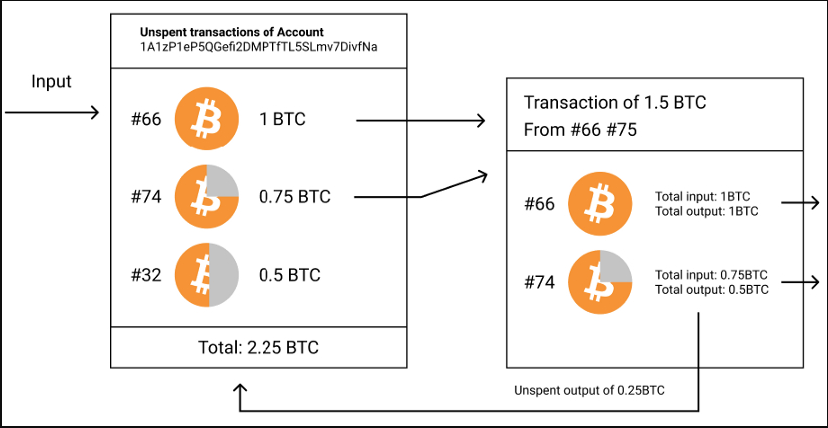
\includegraphics[width=\textwidth,height=6cm,keepaspectratio=true]{utxo_graphic_1.png}
    \caption{
        Sketch of the UTXO transaction format \cite{utxo_graphic1}
    }
\end{figure}

Consider a scenario with three users named Alice, Bob, and Greg.
Greg owns two UTXOs, each valued at 1 Bitcoin.
In total, he owns two bitcoins.
If he wants to send 1.2 bitcoins to Alice and 0.3 to Bob, he puts his two UTXOs into the input field of a newly created transaction.
The input field is already valid since he wants to spend less than he owns.
In addition, Greg must create two new UTXOs in the output field of the transaction to send the money to Alice and Bob.
The first new UTXO contains Alice's public key and the amount of 1.2 bitcoins.
The second new UTXO contains Bob's public key and the amount of 0.3 bitcoins.
Consequently, Greg creates a third UTXO referencing his wallet to receive the remaining value of 0.4 bitcoins as a change, leaving 0.1 bitcoin as a payment fee.

Nevertheless, Satoshi faced a significant problem referenced in his whitepaper.
How could a payee verify that the owner did not spend their coins in an earlier transaction?
This double-spending problem resulted in the need for a mechanism to reach a consensus among all network participants.
The solution had to be cryptographically verifiable and resilient to Sybil attacks or the byzantine fault tolerance problem.
Hence, Satoshi envisioned a distributed timestamping server that kept track of all transactions ever made.
These transactions are collected in so-called blocks.
Each block is a list of transactions. 
Every transaction has a list of input and output UTXOs.
Besides, a block has a timestamped block hash to save the block confirmation date.
Accordingly, all transactions inside a particular block are considered to have happened simultaneously.
Ultimately, a chain of blocks is formed by using the previous block hash as input for the next block hash.
This system is called blockchain and serves as a decentralized solution to the double-spending problem. 

\begin{center}
    \begin{tabular}{|c c c|} 
     \hline
     Problem & Solved & Not Solved \\ [0.5ex] 
     \hline
     Double-spending & \checkmark  & \\ [0.5ex] 
     \hline
    \end{tabular}
\end{center}

\section{Storage management}

Since every new block results in more storage space taken by the software, the constant growth of the blockchain must be limited.
That is why new blocks are created every ten minutes. \cite{nakamoto2008}
Using such a period also ensures the network has enough time to spread a newly found block to all network nodes until the next block is found.

Every block in the chain has a block header that is 80 bytes in size.
It contains the following parts.

\begin{center}
    \begin{tabular}{|c c|} 
     \hline
     Size & Name \\ [0.5ex] 
     \hline
     4 Bytes & Version \\ [0.5ex] 
     \hline
     32 Bytes & Previous block hash \\ [0.5ex] 
     \hline
     32 Bytes & Merkle root hash \\ [0.5ex] 
     \hline
     4 Bytes & Timestamp \\ [0.5ex] 
     \hline
     4 Bytes & nBits \\ [0.5ex] 
     \hline
     4 Bytes & Nonce \\ [0.5ex] 
     \hline
    \end{tabular}
\end{center}

The first four bytes represent the block version. This allows future soft forks to upgrade the block validation rules over time.
Next to them are 32 bytes that contain the previous block hash to ensure the immutability of the chain. This hash is built with the SHA256 algorithm.
A Merkle tree is built to save the transactions inside a block from manipulation. The root of the Merkle tree can be used to validate a particular transaction.
It is 32 bytes in size and also a part of a block header.
The next four bytes are used to store the timestamp, followed by four bytes for the mining difficulty target and four bytes for the mining nonce. \cite{blockheaders}
Mining will be discussed in the Proof of Work chapter of this thesis.

In addition, the number of transactions per block is limited due to a maximum size of one megabyte per block \cite{8215367}.
This results in a maximum potential blockchain growth of:

\begin{equation}
    1MB * 6 * 24 * 365 = 52,560MB = 52.560GB.\textrm{ per year}
\end{equation}

The slow storage increase ensures that running a Bitcoin full node is affordable for everyone, leading to more potential peers on the network. \cite{nakamoto2008}
Consequently, even if a central authority owned thousands of nodes, it would still be unable to control the network because users could still build a node and choose the consensus rules themselves.
Accordingly, when new versions of the software are published, every user who owns a node decides on their own whether to install it.
A new version of the code that would change consensus rules and break compatibility would have to be accepted by nearly every user who runs a node to become a reality in the network. 
This procedure solves the byzantine fault tolerance problem, as every node can verify the transactions independently.
The information is only spread if it is validated. Otherwise, it will be discarded.
\begin{center}
    \begin{tabular}{|c c c|} 
     \hline
     Problem & Solved & Not Solved \\ [0.5ex] 
     \hline
     Byzantine generals problem & \checkmark  & \\ [0.5ex]
     \hline
    \end{tabular}
\end{center}

\section{Proof of Work Consensus}

Reaching consensus in a peer-to-peer network is a challenging problem.
Since the network is freely usable, it must be resilient against bad actors.
Whenever a new block is needed to validate transactions and reach a new network state, someone has to select transactions for the next block and find a valid hash.
Therefore, if a bad actor were to create all upcoming blocks, he could censor specific wallets by excluding their transactions forever.
If it were predetermined who gets to validate the next block, it would leave room for corruption or censorship.
Therefore, the next person to validate a block must be randomly selected.
Satoshi used Adam Backs Hashcash to implement a Proof of Work consensus algorithm to achieve that. 
Each block hash needs to meet specific requirements to be accepted by the network.
Like Hashcash, a miner needs to find a nonce so that the block hash is smaller than a particular target.
The target is chosen by the network and adjusted after every period of 2014 valid blocks.
The adjustment ensures blocks are found every ten minutes on average by raising or lowering the required target for a valid hash.
This process is called difficulty adjustment.

Every miner has a certain probability of finding a valid hash for the block header. 
The more computing power the miner has, the more likely they will be the first to find a valid hash. 
Nevertheless, miners with lower hash rates also have a statistical chance of validating a block. 
If one miner controls 20 percent of the network's hash rate, their chance of finding a valid hash and receiving the block reward is also 20 percent.
This process is comparable to a lottery, where the contributed hash rate is a lottery ticket.
The higher the hash rate, the more lottery tickets.
As a result, it is random who gets to verify the next block based on their hash rate contribution.
However, whenever a new miner joins the network, the percentage of the total network's computing power changes.
Theoretically, a miner that controls at least 50 percent of the network's total hash rate could partially control the mining process by validating more blocks than any other miner.
Consequently, he could censor particular wallets or transactions.
Ultimately, even if any miner reaches this state, they must preserve their power by accumulating more hashing power as the network grows with new miners joining.

Using this technique solved a problem former electronic cash systems faced: the guaranteed inflation of digital money resulting from technological progress and faster computers in the future.
Still, that is not its only purpose.
Satoshi described Proof of Work as one-CPU-one-vote \cite{nakamoto2008}. 
The more leading zero bits it has, the more hashing power it takes to find the hash.
In addition, the block's timestamp further proves how long it took to find it.
Thus, A block's hash proves the global accumulated energy used to validate it because creating the hash took time and consumed energy.

\begin{center}
    \begin{tabular}{|c c c|} 
     \hline
     Problem & Solved & Not Solved \\ [0.5ex] 
     \hline
     Backed by energy & \checkmark & \\ [0.5ex] 
     \hline
    \end{tabular}
\end{center}

If a new computer is to enter the network, it needs to receive the chain from other peers.
Without Proof of Work, malicious peers could create fake chains and send them to new nodes.
Only the network difficulty and the block hash provide information that makes identifying the honest chain possible.
The chain with the greatest difficulty and, thus, the highest computational effort is most likely the honest chain \cite{nakamoto2008}.

In theory, creating a fake chain is only possible if one has more hashing power than the honest part of the network.
First, an attacker would have to recalculate all blocks that happened since the block they want to fake.
Then, they must calculate new blocks faster than the rest of the network to convince the network nodes that the fake chain is the honest chain.
If two chains exist in parallel, every network node will choose the faster-growing chain with the same difficulty and discard the other.
Thus, a central authority could only take over the consensus algorithm if it had more energy and hardware in control than the rest.
The Sybil attack is prevented by making it uneconomical and difficult to perform a system takeover.
\begin{center}
    \begin{tabular}{|c c c|} 
     \hline
     Problem & Solved & Not Solved \\ [0.5ex] 
     \hline
     Sybil attacks & \checkmark  & \\ [0.5ex]
     \hline
    \end{tabular}
\end{center}

Furthermore, the chain uses the Proof of Work consensus mechanism to issue new coins into the ecosystem.
Whenever miners find a valid block hash, they receive a transaction that pays a so-called block reward consisting of newly created coins and transaction fees.
In turn, miners are incentivized to secure the network with their hashing power, while the amount of new coins rewarded is halved every 210,000 blocks to prevent money supply inflation.
As a result, there is an upper supply limit of nearly 21 million bitcoins.
Bitcoin uses Proof of Work to solve the double-spending problem and to issue new coins into the system without the risk of hyperinflation or a central authority controlling the supply \cite{wirdum_2_2018}. 


\begin{center}
    \begin{tabular}{|c c c|} 
     \hline
     Problem & Solved & Not Solved \\ [0.5ex] 
     \hline
     Inflation resistant & \checkmark & \\ [0.5ex] 
     \hline
    \end{tabular}
\end{center}
\newpage
\section{Nodes}

Bitcoin is a peer-to-peer network consisting of computer nodes running the Bitcoin program.
There are four different types of node programs in total that serve different purposes.

\begin{itemize}
    \item Full node
    \item Header-only node
    \item Signing only (Wallet)
    \item Mining nodes
\end{itemize}

\textbf{Full nodes} run the original Bitcoin software. 
Thus, they include all protocol functionalities and keep a full copy of the blockchain.
Their main task is to verify incoming transactions or newly found blocks from the miners. 
If a block is valid, they propagate it to other nodes to spread the information through the network.
In addition, they also store a full copy of the blockchain.
The first user-friendly program to interact with the Bitcoin blockchain was the Satoshi Client, named after the Bitcoin creator.
It had a wallet address and private key to sign and receive transactions and could also participate in mining.
Yet, the mining capability was removed to build a separate, more efficient mining client. \cite{skudnov2012bitcoin}

Next to full nodes, Satoshi introduced another client that could verify transactions without a full blockchain copy.
These clients are called \textbf{header-only nodes}.
As the name suggests, it only stores the block headers without knowing a block's transactions.
It only knows the Merkle tree root hash that contains all transactions.
Hence, it relies on full nodes sending block headers to the client.
To prevent some malicious full node from sending a manipulated block header, it asks different nodes until it has found the longest Proof of Work chain.
As already stated, the difficulty of each block suggests how much effort went into computing the whole chain, which acts as proof of energy consumption. 
Since these nodes do not store a local copy of the blockchain, they are only partially trustless like a full node.
Regardless of being unable to verify new transactions, they can still tell if a particular transaction has happened by calculating whether the Merkle tree root of the transactions in the blocks header contains a particular transaction hash. \cite{nakamoto2008}

Besides these two implementations, there are also \textbf{signing-only clients}.
They do not even store block headers but only possess a private key.
Accordingly, they can only sign new transactions and keep a local copy of their transaction history. 

The fourth client is called \textbf{mining client}.
While initially implemented into the Satoshi Client, they were replaced by more efficient clients using the GPU to achieve more hashes per second.
The more hashes a client can generate, the higher the chances of finding a valid hash in the Proof of Work consensus algorithm. \cite{skudnov2012bitcoin}

However, more than GPUs are needed to find a valid block today.
Over the years, special mining hardware capable of hash rates up to 100 terra hashes per second was designed by several companies, such as Bitmain. \cite{bitmain_shop}
Nevertheless, even with this kind of specialized hardware, it is doubtful for one device to find a valid block hash.
That is why a concept called pool mining emerged over time.
Instead of mining as a single entity, many miners worldwide try to find a valid block hash together.
Whenever a valid block is found, all participants get a share according to their hash rate contribution.
It is comparable to lottery players splitting the prize whenever any player wins something. \cite{lewenberg2015bitcoin} 
According to hashrateindex.com \cite{hashrate}, the mining pools with the greatest hashrates are Foundry USA with 30.1\% and AntPool with 26.2\%.

\chapter{Ethereum and Smart Contracts}
The Ethereum blockchain allows code execution designed in a smart contract language like \textbf{Solidity}. 
As a result, a game can execute primarily defined methods of the smart contract. 
Using these contracts makes it possible to store in-game items, weapons, or character statistics on Ethereum. \cite{buterin2014}

\section{Ethereum Virtual Machine}
Like Bitcoin, Ethereum is a decentralized network that agrees on a network state.
A state is a collection of accounts with a 20-byte address.
Every account stores its Ether balance, a contract code if one was provided in bytecode form, and a contract storage, which is divided into three types.
First, there is long-term storage that uses key-value pairs to store data.
To create variables temporarily, developers can use the stack or the memory.

Further, two types of accounts are described. The first one is a standard user account controlled with a private key. 
They only issue external transactions, meaning transactions from outside the blockchain.
The second one is a contract account that controls its smart contract. 
They can also issue internal transactions from one smart contract to another.
Receiving a transaction as a contract account always leads to a code execution and, thus, to a state change. \cite{ethereum_virtual_machine}
The fact that the blockchain executes Turing-complete code leads to the term \textbf{Ethereum Virtual Machine} because the network acts as one computer system.

However, code execution does not happen instantaneously. 
Like regular transactions, a code execution transaction needs verification in a block.
Thus, standard money transfers and code executions compete for block space, resulting in transaction fees, called gas, measured in wei. 
One wei equals 0.000000000000000001 Ether.
Depending on the network usage, the cost of gas changes.
In addition, a user can provide a gas limit when issuing a transaction to prevent unintended execution of poorly programmed smart contracts.
As a result, developers of smart contracts are heavily incentivized to write high-performance code that uses storage effectively.
Consequently, infinite loops are avoided. 
Crashing the whole network would cost a tremendous amount of Ether, which makes it a wasteful effort.

\section{Smart Contracts in Game Development}
Since the EVM bytecode is Turing-complete, many different things can be done using programming languages like Solidity.
This chapter will show some approaches to implementing game-related data using Solidity, the most commonly used smart contract language.
It is a high-level, object-oriented, statically typed programming language.
It supports various concepts of object-oriented programming, such as inheritance, interfaces, abstract classes, and structures.

\clearpage
\subsection{Smart Contract Implementation: Virtual Pets}

\begin{framed}
\textbf{Implementation: } Virtual Pet \medskip \hrule \medskip
\textbf{Used Contract: } ERC-721 Non-Fungible Token Standard\medskip \hrule \medskip
\textbf{Details:}  This example shows how to implement so-called Virtual Pets using Solidity.
The contract is based on the ERC-721 NFT standard. 
Everyone can create a new pet by using the createNewPet() function.
The function mints a new ERC-721 token and randomly draws properties for the new pet.
\end{framed}
First, some pet properties are defined in the contract.
\lstinputlisting[language=Solidity,linerange={3-16}, caption=Solidity pet properties, label=Solidity pet properties]{listings/VirtualPet.sol}

However, every pet should have different properties, so functions to generate them randomly are needed.
In addition, pet sizes should have different probabilities.
\lstinputlisting[language=Solidity,linerange={43-54}, caption=Solidty pet property creation, label=Solidty pet property creation]{listings/VirtualPet.sol}
\lstinputlisting[language=Solidity,linerange={56-67}, caption=Solidty pet property random function, label=Solidty pet property random function]{listings/VirtualPet.sol}

The random number functions used for this example are deterministic due to the nature of the EVM not having any byte code functionality to create true randomness.
\lstinputlisting[language=Solidity,linerange={71-78}, caption=Solidity random functions, label=Solidity random functions]{listings/VirtualPet.sol}

Finally, a function to create a new pet is implemented. 
In addition, a function to obtain the pet properties is also needed so they can be used in a game.
\lstinputlisting[language=Solidity,linerange={18-35}, caption=Solidty pet creation function, label=Solidty pet creation function]{listings/VirtualPet.sol}
\newpage
Then, a getter for external function calls from the Unity game implementation is created.
\lstinputlisting[language=Solidity,linerange={36-39}, caption=Solidity pet property getter, label=Solidity pet property getter]{listings/VirtualPet.sol}
\clearpage

\subsection{Unity Implementation: Using Virtual Pets in a Game}
After publishing the virtual pet smart contract on an EVM blockchain like Ethereum, a game engine like Unity can communicate with it.
For this purpose, the Thirdweb SDK will be used \cite{thirdweb_sdk}.

Code to set up the player wallet for further smart contract interactions.
\lstinputlisting[language={[Sharp]C},linerange={3-20},caption=Setup Code, label=Setup Code]{listings/UnityImplementation.cs}

Example code to call a read function on the smart contract and do something afterward.
\lstinputlisting[language={[Sharp]C},linerange={22-29},caption=Read interaction, label=Read interaction]{listings/UnityImplementation.cs}

\newpage
Example code to call a write function on the smart contract and do something afterward.
\lstinputlisting[language={[Sharp]C},linerange={31-39},caption=Write Interaction, label=Write Interaction]{listings/UnityImplementation.cs}

Helper function to obtain an object representation of the smart contract.
\lstinputlisting[language={[Sharp]C},linerange={43-46},caption=Smart contract loading, label=Smart contract loading]{listings/UnityImplementation.cs}

Helper function to call the getPetProperties() function of the smart contract.
\lstinputlisting[language={[Sharp]C},linerange={48-51},caption=Get per properties, label=Get per properties]{listings/UnityImplementation.cs}

Helper function to call the createNewPet() function of the smart contract.
\lstinputlisting[language={[Sharp]C},linerange={53-56},caption=Call create new pet function, label=Call create new pet function]{listings/UnityImplementation.cs}
\chapter{Evaluation: Blockchain and Games}

Besides the technical possibilities that result from inventions such as Ethereum, what they are useful for is questionable.
The blockchain was initially designed to solve the problems of digital money proposed earlier. 
Ethereum then created a blockchain that could execute Turing-complete code instead of simple operation codes.
According to the Ethereum whitepaper, the use case is that decentralized apps or organizations could be built using smart contracts.
However, are these apps decentralized? What are the benefits or drawbacks? 

\section{Difference between Bitcoin and Ethereum}
Although Ethereum is also based on a blockchain, Bitcoin has critical differences. \cite{Arslanian2022}
Some of them lead to the question: Is Ethereum decentralized?
This chapter will first show the differences and afterward present some arguments for and against Ethereum.

First, there are technical differences.
Besides the fact that Ethereum can run Turing-complete smart contracts, it also has a much shorter block time of only 17 seconds compared to Bitcoin's ten-minute block time.
While Ethereum was initially launched with Proof of Work, the consensus was changed to \textbf{Proof of Stake} in 2022. \cite{ethereum_merge}
Proof of Stake does not rely on finding partial hash collisions. Instead, nodes are selected to verify the next block based on a staked amount of Ether compared to the total staked amount in the network. 
This amount is locked inside a smart contract and serves as insurance against fraudulent behavior. \cite{proof_of_stake}
Earlier in this thesis, a significant problem that comes with the absence of Proof of Work was discussed.
New nodes joining the network require other nodes to send them the honest chain. 
However, without Proof of Work, a node cannot verify that it received the honest chain.
In a proof of work context, the honest chain is described as the one with the greatest difficulty, resulting from the fact that an attacker cannot compute a fake chain faster than the rest of the network \cite{nakamoto2008}.  

A second consequence of Proof of Stake is the centralization of power and wealth. While Proof of Work needs the miner to constantly compete with the rest of the network, Proof of Stake lacks this mechanism.
The node with the highest stake has the highest chance of verifying blocks and thus receives most of the block reward. 
Consequently, the node could stake the Ether it gets to preserve its power in the network.
The more coins it has, the more power it has in the network. 

Another problem leading to centralized Proof of Stake is that a minimum amount of Ether must be locked to participate in the consensus.
By requiring a minimum amount, only some users can participate in the consensus mechanism.
Only those who have enough Ether can start staking.
However, central services, including crypto exchanges, offer staking services to customers who cannot afford the minimum amount.
This results in the service controlling the staking nodes and the network consensus.
In contrast, in the Proof of Work consensus, everyone can participate with every hardware that can execute the SHA256 algorithm.
Thus, third parties are not needed, which prevents centralization.
Accordingly, centralizing Proof of Work is more difficult because it relies on a central authority being more energy and resource-efficient than the rest of the network.
Proof of Stake centralization is possible, with users giving their coins to these services to participate in the mechanism.

However, there are also social differences between Ethereum and Bitcoin.
When looking at the first days of Ethereum, one significant difference is that Ethereum was initially funded via a presale.
This event led to the creation of a significant amount of Ether that was sold to selected investors.
In contrast, the Bitcoin software was published before Nakamoto announced the start of the network.
Technically, everyone had the opportunity to participate in the Bitcoin network from day one. 
Nakamoto never created coins without doing the Proof of Work on his machine.
By doing this presale, the Ethereum Foundation took a position with significant influence on the network.
Investors that bought Ether from the Foundation expect the Foundation to create the network they announced.
Hence, when the Foundation decides to take a different path and change the software, many investors would potentially follow their decision. \cite{eth_presale}

Although Bitcoin and Ethereum are designed to be decentralized networks, we conclude that preserving this state is more of a \textbf{social consensus}.
The narrative and idea of the concept play an essential role. 
As a result, a decentralized network must also be socially decentralized, meaning that no central entity has enough influence to change the network or influence the network's majority on its own.
This is one of the reasons why Nakamoto left the Bitcoin project in its early days. 
As the creator of the initial protocol, he had a social influence on the network. 

An event that further strengthened the critique of the role of the Ethereum Foundation was the \textbf{DAO hack} in 2016 \cite{dao_hack}.
The hack used a so-called reentrancy attack that requires an attacking contract and a vulnerable smart contract.

The following code snippets are taken from \cite{reentrency_attack_snippets}.
In order to perform the attack, two functions need to be set up.
First, the attack function deposits and withdraws funds.
\lstinputlisting[language=Solidity,linerange={15-19}, caption=Attack function, label=Attack function]{listings/Attack.sol}

The vulnerability can be found in the withdrawal function of the vulnerable contract.
The caller of the function first receives their funds, and then the contract's internal balance of the caller is updated.
However, the caller is a smart contract that changed their fallback function, which is called whenever a payment is received.
\lstinputlisting[language=Solidity,linerange={8-16}, caption=Vulnerable withdraw function, label=Vulnerable withdraw function]{listings/DepositFunds.sol}
The attacking contract now calls the withdraw function again, resulting in a recursion that makes the vulnerable contract send funds to the attacker while never updating its internal balance.
\lstinputlisting[language=Solidity,linerange={9-13}, caption=Attackers fallback function, label=Attackers fallback function]{listings/Attack.sol}
This attack is easily prevented by first updating the caller's balance and then sending the funds.

Vitalik Buterin proposed a soft fork to censor the attacker's wallets in response to this hack.
However, because of a software vulnerability in the soft fork, a hard fork was proposed instead, which would roll back the blockchain to an earlier state.
Due to the protocol's technical decentralization, Vitalik could not force the hard fork by himself. However, the node operators and miners agreed to update their software.
Consequently, the impact of the Ethereum Foundation on this network decision should be questioned. 
Without the Foundation initially proposing a fork, it might have never led to that outcome.
Besides, the DAO hack was not the consequence of a bug in the Ethereum blockchain. Instead, it was a software bug in the DAO's smart contract. 
According to the attacker, he technically just used the smart contract functionalities and did not commit a crime. \cite{dao_hack}
The rollback of the blockchain broke the narrative of it being immutable. Payments that had already been made were removed from the chain.

A second event that split the Ethereum community again was the so-called \textbf{merge}, which changed the network's consensus rules from Proof of Work to Proof of Stake.
It is questionable whether such decisions would become a reality without the influence of the Ethereum Foundation. 

As a result, Ethereum's narrative and use case is very different from that of Bitcoin.
Accordingly, Ethereum cannot replace Bitcoin, which is often claimed to happen in the future \cite{flippening_2023}.
Given the threat of potential rollbacks or changes in the network rules, it does not work as a digital store of value, such as Bitcoin. 
However, it has the Turing-complete smart contract functionality, which Bitcoin lacks.

\section{The oracle problem}
The last chapter concluded that Ethereum serves a different purpose than Bitcoin. 
This thesis also worked out that the purpose of blockchain technology is to solve the problems of digital cash.
Before making a statement about the use case of smart contracts on Ethereum, the so-called \textbf{oracle problem} has to be defined.
The term \textbf{oracle} first appeared in a paper by Alan Turing in 1937 \cite{turing1939systems}. 
It described a black box that provided noncomputable information to a Turing machine.
In 1978, William Howden stated in \cite{10.1109/TSE.1978.231514} that software testing also needs oracles.
According to Howden, a software test relies on an oracle to tell whether it has passed.
Usually, this oracle is portrayed by a human being, a programmer, who checks if the tests are implemented correctly and produce correct results.

If real-world assets such as gold are traded digitally, they are represented by certificates that promise that the respective asset backs them.
However, only an oracle, in this case, the bank that stores the gold, can assure that it is in their possession. 
As a regular owner of such certificates, they have no option but to trust the bank because they cannot enter the bank's safe and check on themselves.

In conclusion, an oracle is an abstract entity that provides information.
The problem is that it must be trusted whenever the oracle provides data.
It is further complicated to audit the data repeatedly to verify their integrity. 
Besides, an auditor would be an oracle as well.

Bitcoin solves this problem by not implementing it in the first place.
The Proof of Work serves as proof of energy consumption, resulting in a digital representation of a natural resource.
No oracle is needed to prove the work, making the blockchain trustless. 
This detail causes many discussions about using the blockchain to store data about supply chains \cite{blockchain_supply_chains}, health care \cite{blockchain_healthcare}, or video game data.
However, storing external data on a blockchain does not guarantee integrity.
Besides, the initial use case of stored data is subject to change in the future.

Giulio Caldarelli discussed the blockchain oracle problem in \cite{info11110509}.
He concluded that oracles are the only way to provide data integrity for external data stored in a blockchain.
Besides, oracles are most often centralized and can be compromised or manipulated.
While the impact and the possible damage depend on the data, it is still a relevant problem that requires further research.
In addition, the author proposes new questions that need a proper answer before using the blockchain in various areas.

\begin{quote}
	\textit{
		SUPPLY CHAIN: Can a firm reputation alone counter the oracle problem? If oracles are unable to prevent the upload of unwanted information, who will benefit from blockchain implementation?
		}
		
	\textit{
		HEALTHCARE: Can patients themselves be oracles? Can a distributed system also guarantee privacy and security?
		}
		
   \textit{
   		LAW: What is the legal role of oracles? How can smart contracts be enforceable? How does one prevent illegal smart contracts? 
   }
   \cite{info11110509}
\end{quote}

\section{Blockchain as a Buzzword} 
The invention of smart contracts on blockchains, namely Ethereum, led to many games that utilized this technology.
One of the first games to actively integrate NFTs and cryptocurrencies was Cryptokitties. The game launched in late 2017 and was published by Dapper Labs. \cite{serada2021}
According to their whitepaper, one of their main goals is to make blockchain technology more accessible for the average person.
Although the game is marketed as a blockchain game, it has no direct gameplay.
It occurs on the Cryptokitties website, where the user has to buy, breed, and sell cats.
Consequently, the game is more comparable to a card-collecting game than a classical video game.
According to the Cryptokitties team, using digital collectibles in games has vast potential for the gaming industry. 
However, they identified why these digital items failed to succeed.
First, they cannot rely on a trusted third party to issue them. 
Second, their functionality should be independent of the founder's existence. 
What is the purpose of a digital collectible when the issuer turns off the servers and makes them inaccessible? \cite{cryptokitties2017}
These statements are very close to what Szabo concluded in his paper about Third parties being security holes \cite{szabo2001}.

Nevertheless, there are a few contradictions between the Cryptokittie's whitepaper and how the game is implemented.
One can be seen in the smart contracts developed for the game. \cite{source_cryptokitties_2017}
Some specific wallet addresses are granted administrative permissions in the code.
Explicit function modifiers make certain functions exclusively executable by these addresses. 
As a result, Dapper Labs could interfere with the Cryptokittie's ecosystem and break the promise of digital scarcity by creating new kitties. 
They could even upgrade or replace the existing contracts entirely.
Moreover, the pictures of the cats are neither stored nor created on the blockchain. 
Without the official Cryptokitties website and its central services, the cats would lose their personality without these pictures. 
This would be comparable to a Pokemon card losing the image of the Pokemon.
Hence, the game depends on its maintenance by the publisher.

In summary, the development team concludes that digital collectibles should not depend on the creator but implement such dependencies into the game's code.
The blockchain makes the peer-to-peer transfer of kitties possible.
However, the only solution it provides is preventing double-spending without relying on a trusted third party. 
Since the game, by design, relies on the founder, a trusted third party is still needed, thus making the blockchain obsolete.
By choosing blockchain as a database, the ecosystem benefits from blockchain functionality at the expense of scalability and immutability of data.
According to \cite{jiang2021}, these limitations led to the game's failure.

In 2018, another blockchain game was released that was heavily inspired by Cryptokitties. 
It was named Axie Infinity and was published by Sky Mavis.
The game also relied on collectible entities. 
This time, they were called Axies, which could be used to fight against other players' Axies.
This so-called \textbf{Play-To-Earn concept} would reward their players with Axie Infinity's cryptocurrency AXS.
Sky Mavis then implemented the Ronin Sidechain because of the number of smart contract calls executed daily to keep the game running.
A sidechain runs parallel to a main blockchain while implementing different consensus rules, block size limits, and transaction speeds. \cite{axie_analysis}
In 2021, the game reached significant popularity.
With the rising price of the cryptocurrency, it became more difficult to join the game since playing requires a player to own Axies, which are priced in AXS.
Thus, a scholarship program was implemented that added the functionality to borrow Axies from other players.
Consequently, the early players that already owned Axies lent them to new players, made them play the game, and gave them a small fraction of the earnings.
Especially in poor countries such as the Philippines, players depended on their Axie-lenders and the game.
However, the value of AXS dropped significantly in 2022.
In addition, the bridge between the Ronin Sidechain and the Ethereum Blockchain was hacked in March of 2022 \cite{axie_collapse}.
The hacker stole about 600 million dollars worth of mostly user funds.
Therefore, many players who invested in the game to play it and reach a better financial situation lost everything. \cite{axie_article}

Given that a central software to run such games would be a better alternative, the usage of a blockchain works marketing-wise but not from a software engineering perspective.
In addition, the Play-To-Earn concept of Axie Infinity, which is possible through blockchain infrastructure, created a Ponzi scheme.
Accordingly, the players who owned Axies got richer until they sold their assets, leaving worthless Axies and desperate Axie borrowers behind.
This conclusion begs the question, what are the benefits of using a blockchain compared to central services?

\section{Problems of Smart Contracts for Software Engineering}

\subsection{Problem: Randomness}

Since Solidity is executed on a blockchain, there is one problem a programmer might face when implementing game data, meaning randomness.
This problem was further discussed in~\cite{8751326}.
The reason for this is that smart contracts are deterministic due to the nature of the blockchain.
Since all nodes that execute the smart contract code must reach consensus, byte-code does not support random number generation.
Although, there are some approaches to achieving deterministic randomness.
While they are unsuitable for sensitive algorithms such as casinos or financial systems, they might be enough for game data.

The first approach is to use an oracle. 
As already described in this thesis, oracles are external sources of data a blockchain can use.
Since the Oracle code is not performed on the blockchain, it cannot be manipulated. 
However, the oracle is also a security risk since it is compromisable.

A second way to generate random numbers is to use information from the current block.
An example of this can be seen below.
It uses the hash function keccak256 and the abi interface to encode the data to minimal using space data.
A deterministic number will be created using block data and the contract caller's address.
In addition, a random number seed is also provided.
\lstinputlisting[language=Solidity,linerange={1-40}, caption=Deterministic random number generation in Solidity, label=Deterministic random number generation in Solidity]{listings/random.sol}

\subsection{Problem: Immutability}
Another critical problem that contrasts with modern software engineering concepts is the immutability of smart contracts.
Software engineering is a fluent process of implementing features and fixing bugs that occur when testing the application.
However, it is not sure whether an application is bug-free.
Since smart contracts are often used in a context where wallets own specific assets or rights, making them as secure as possible is crucial.
This makes the threat of potential hacking attempts severe since there is much incentive to steal valuable user funds.
In addition to intentionally exploiting code vulnerabilities, there is also the possibility of bugs not being found during the testing process.

OpenZeppelin, a software company specializing in smart contract development, proposed a solution to this problem. \cite{zeppelin_proxy}.
They described a proxy upgrade pattern.
A proxy contract would be used to delegate calls to a logic contract.
The benefit of this design is that the logic contract can be swapped in the background.
The user will constantly interact with the proxy.
Thus, the contract address of the proxy always stays the same.
However, implementing such a concept takes time and effort.
First, there are potential storage collisions resulting.
A storage collision occurs when both the proxy and the implementation use the same address in storage to store their data.



In this example, the proxy stores the implementation address in the same variable slot where the implementation contract stores an address.
To counter this, OpenZeppelin proposed a concept called "unstructured storage," where a random slot is chosen for the proxy variable to ensure no collisions.
\begin{figure}[htpb]
   \centering
   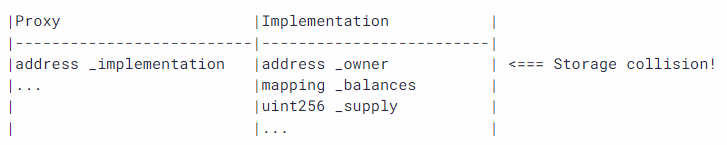
\includegraphics[width=\textwidth,height=6cm,keepaspectratio=true]{collision_1.png}
   \caption{
       A storage collision between proxy and logic data \cite{zeppelin_proxy}
   }
\end{figure}


Another example from OpenZeppelin shows how a collision happens when a contract upgrade is not performed correctly.
The order of variables inside the source code must be preserved.
If not done correctly, the already saved data clashes with the new field saved at that particular slot.
\begin{figure}[htpb]
   \centering
   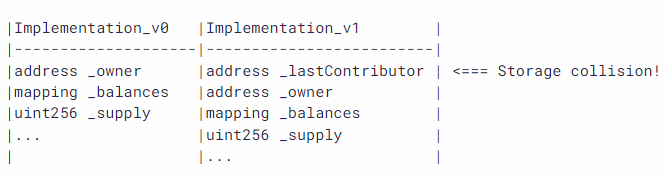
\includegraphics[width=\textwidth,height=6cm,keepaspectratio=true]{version_collision.png}
   \caption{
       A storage collision after a contract update \cite{zeppelin_proxy}
   }
\end{figure}

In addition to storage collisions, there are also function clashes.
They are described as two functions named the same or sharing the same 4-byte code identifier, resulting in a collision.
A transparent proxy solves this issue by picking the function based on the address of the function caller.

\begin{quote}
\centering 
   \textit{If the caller is the admin of the proxy (the address with rights to upgrade the proxy), then the proxy will not delegate any calls and will only answer any messages it understands.}
   \textit{If the caller has any other address, it will always delegate a call, whether it matches one of the proxy's functions.} \cite{zeppelin_proxy}
\end{quote}


\subsection{Problem: Blockchain Scalability}
Blockchains' scalability issues come with using blockchains to store external data or execute smart contract logic.
Every state-changing action requires a transaction, while all transactions compete for block space with fees.
The Bitcoin blockchain processes about seven transactions per second, which is neither suitable as a protocol to use for daily transactions nor would that grant
sufficient speed for code execution. Ethereum already has a block time of a few seconds compared to Bitcoin's block time of ten minutes.
Yang, Long, Xu, and Peng analyzed the scalability problem of blockchains in \cite{blockchain_scalability} and named potential solutions.

One of these solutions is called \textbf{Sharding}. 
A concept initially designed to split large databases into smaller ones to distribute the workload and enhance efficiency.
In the blockchain context, smaller chains, called shards, produce blocks that are appended to the main chain.
While this process allows for faster transaction speeds and improved network performance, some drawbacks could lead to potential security problems.
One of them is a Single Shard Takeover Attack. 
Taking over the Bitcoin blockchain requires an attacker to have more processing power than the rest of the network.
However, taking over a shard requires a percentage of the original amount.
Besides, managing the shards and efficiently balancing the workloads requires complex code that could lead to new vulnerabilities and bugs. \cite{sharding_binance}

Another concept is the use of off-chain payment networks.
Instead of changing the blockchain or its consensus rules, the use of the protocol is changed.
Accordingly, the underlying blockchain serves as a settlement base layer.
Smaller transactions are performed in the payment network.
The settlement is done by publishing one transaction containing billions of off-chain transactions.
One example of such a network is the \textbf{Bitcoin Lightning network} \cite{poon2016}.
It creates multi-signature wallets between two parties that serve as payment channels.
Transactions between these two entities are not tracked on-chain. 
Instead, the settlement transaction is done when closing the channel. 
As a result, network channels can be used to route payments through the network.
If Alice has a payment channel with Bob and Bob has a channel with Tom, Alice can send funds to Tom.
However, the network also comes with some drawbacks.
Since two parties share a payment channel, users are advised to keep their lightning node online to prevent fraudulent behavior.
Else, it would be possible to steal funds from the channel.
Besides, the network needs liquidity to route payments. 
If Alice wants to send 0.5 bitcoin to Tom, but the channel between Tom and Bob does not have 0.5 bitcoin for routing, it cannot be done.
The only way to transfer liquidity into the network is by issuing main-chain transactions to lock the coins into a payment channel.

Besides the Lightning network, there are other implementations for other blockchains, further described in \cite{blockchain_scalability}.
While there are more solutions for the scalability problem, more scalability always comes with drawbacks.
This consequence is called \textbf{blockchain trilemma} \cite{blockchain_trilemma}, meaning the trade-off between decentralization, security, and scalability.
Bitcoin was designed concerning decentralization and security, resulting in a low transaction speed and, thus, less scalability.
This design choice serves the narrative of a blockchain being a secure payment network without relying on a trusted third party.
As a result, using blockchains to store data or execute code is always limited by blockchain technology.
The chain would lose its initial purpose if a scaling solution leading to less decentralization or security problems were used.
Hence, using blockchains over centralized services will always be less efficient.

\section{Opportunities of Smart Contracts for Software Engineering}
Besides these drawbacks, there are also opportunities.
Before evaluating these arguments, it is crucial to note that every argument for blockchains and smart contract usage should exclude any oracles or third parties.
Otherwise, the blockchain would lose the decentralization features it was made for, while the software engineering problems would stay.
When implementing solutions or concepts using smart contracts, the Oracle problem is the most crucial question to ask.
Even if a full game or program is implemented using only smart contracts, the programmer might always have special administrative rights to control certain contract parts.
For example, the administrator could issue virtual items with admin functions instead of using the normal contract functions. Alternatively, some variables of the contract could be changed.
If not fully solved or even addressed, centralized services will always be a better design choice to implement data or code logic.

\subsection{Opportunity: Code Transparency}
Due to the nature of public blockchains, all data is available for everyone at any time.
Hence, all smart contracts and their byte code are public as well.
This transparency could be used as a feature to implement specific game program codes into the chain, such as random number generators for loot drops or crucial game mechanics.
However, it is not guaranteed that any game uses these contracts.
Furthermore, the company producing a game could change its source code and not use smart contracts anymore.
Thus, users again face the oracle problem.
However, the argument might be valid if the whole game is programmed with smart contracts, with all the software engineering drawbacks.
Games that use this approach can only implement a few game mechanics due to the scalability issues. \cite{8848111}

\subsection{Opportunity: Code Reusability}
Since anyone can execute smart contracts, different games can use them simultaneously.
Character stats or virtual items could be beneficial in different games. 
In addition, if more than one game uses the virtual item, the value is not dependent on only one-third party.
While this argument does not solve the oracle problem, it at least distributes the counterparty risk to many third parties. \cite{8848111}

Besides, using existing code and a functioning blockchain reduces the workload.
With blockchains, an existing infrastructure that requires neither maintenance nor running costs can be used.
When game items or logic are already implemented on the chain, games can adopt them and connect their product to an existing ecosystem. 
However, the oracle problem will always be a part of these solutions, which results in the question of whether centralized services would also work
to achieve the same outcome.
\chapter{Conclusion}
Blockchain technology was created to solve problems many digital cash protocols failed on.
After years of research and proposals of several Cypherpunks, Satoshi Nakamoto presented a whitepaper about Bitcoin.
The main feature of this solution is a decentralized peer-to-peer network that does not rely on any third party.
Accordingly, it was designed only to process seven transactions per second to focus on decentralization and security in the blockchain trilemma.
Every attempt to change the blockchain design by other projects like Ethereum to achieve more scalability leads to less security or centralization.
However, both are needed to make the chain a tamper-proof digital cash solution, which it was designed for.
Further, the social consensus of the Bitcoin network is the backbone of its value proposition.
The decentralized open-source character, the origin story, and its network effects differentiate it from every other cryptocurrency implemented afterward.
If other cryptocurrency and blockchain implementations do not contribute any improvements, they might just be trying to imitate Bitcoin and its narrative for marketing purposes.

As a closed ecosystem, the blockchain only contains data secured by its consensus rules.
Accordingly, it cannot prove the integrity of external data in any way.
This so-called blockchain oracle problem leads to data only being valid when an oracle grants its validity.
Ingame items on the blockchain are only valuable if the game's code uses them. 
If an entity does not abide by the terms of a smart contract, it always needs an external authority to enforce it.
In addition, there is no guarantee that a smart contract that is created today will be used for its initial purpose tomorrow.
Consequently, third parties are needed again, even though the entire technology should exclude them, and therefore, they must accept significant disadvantages to achieve that.
These drawbacks also come into play when using smart contracts instead of a centralized database to store game-related data. 
Although there are some benefits, it is questionable whether they are significant enough to justify the software engineering problems that come with them.

As a result, we conclude that blockchain technology is a superb implementation for solving the problems of digital cash.
However, we do not see any use case for blockchains as a distributed database to store external data.
The only data that should be stored on a blockchain is data that was created through a decentralized consensus that is very hard to compromise.
Proof of Stake removes the thermodynamical properties provided by Proof of Work, making it impossible to identify the honest chain by its mining difficulty.
Therefore, blockchain networks, namely Ethereum, that use the Proof of Stake consensus algorithm cannot store digital wealth.
While it is primarily used to execute smart contracts, which are subject to the Oracle problem, it is even questionable whether Ethereum was designed to solve an existing problem or if the need for smart contracts in a blockchain was constructed to justify Ethereum's existence.
\chapter{Future Work}

This thesis might serve as a foundation to further expand on what blockchains can be used for.
While storing external data on a blockchain does not guarantee the truthfulness of the information, there might still be other use cases for blockchains.
We propose a different view to concentrate on second-layer solutions that do not change a blockchain or store any third-party information directly.
Instead, layer two protocols could use the blockchain as a distributed timestamping server, which it was initially called by Nakamoto \cite{nakamoto2008}, or as a base layer to prove the state of their network.
These layers could also choose a more scalable design since the underlying chain is still secure.
Storing third-party data on these new systems has no drawbacks like storing them on the main chain, making it a better software engineering approach.

\section{Scaling Bitcoin with the Lightning Network}
The Bitcoin Blockchain creates a fundament for a whole new ecosystem to be built on top. 
Since its first launch over a decade ago, new systems have been created with Bitcoin as a base settlement layer.
One of them is the Bitcoin Lightning network \cite{poon2016}, which is capable of routing payments through a network of payment channels that are settled on the Bitcoin blockchain.
Every payment channel is a wallet that is controlled by two entities. 
They can transfer coins inside this channel without waiting for the Bitcoin blockchain to verify it in a new block. 
This results in billions of daily transactions compared to about seven transactions per second on the blockchain. 
Thus, games could use Bitcoin Lightning as an alternative to a traditional payment infrastructure for micro-payments.

\section{Trusted Timestamping}
Timestamping is used to prove data's existence at a particular moment.
Thus, the services that provide such timestamps must be trustworthy.
In addition, the timestamps must be cryptographically saved from being altered afterward.
That is where Bitcoin could play an essential role as a distributed time-stamping server.
The idea of using the Bitcoin blockchain like that is further discussed in \cite{timestamping}.
The author proposes to store hashes of documents or data on the Bitcoin blockchain, which proves the existence of the data at the time of the block validation.
As already discussed, storing data on the main chain comes with drawbacks.
However, the only property a blockchain can prove about third-party data is when it was stored.
If this is the only property needed and the transaction costs are worth the data, it might be a valid use case that needs further research.

\section{BitVM}
Instead of storing data directly on a blockchain, BitVM could be used as a second layer that replaces implementations like Ethereum.
We have already concluded that smart contracts on the Ethereum platform are subject to its scalability issues.
Further, the contracts need oracles in most cases, creating a contradiction between the initial idea of excluding third parties and the need for trusted data providers and contract enforcers.
However, when a second layer is used instead, the software engineering drawbacks are not a problem anymore.
While the use case of smart contracts is still questionable, the blockchain is no longer used to execute them.
Second-layer smart contract platforms might serve new application areas that need to be discovered by further research in this field.

\backmatter
% optional: list of figures
\listoffigures
% optional: list of tables
%\listoftables
% optional: list of source code listings
\lstlistoflistings

% your BibTex file
\bibliography{bib/references.bib}


%\appendix
% include appendix chapters here

% \chapter{Appendix A}
\section{Software Framework Documentation}\label{sec:FrameworkDoc}

\lipsum[1-2]


\lstinputlisting[language=C++,caption=Example code snippet, label=HelloWorld_listing]{listings/HelloWorld.cpp}


\end{document}
